\chapter{Конструкторская часть}

\section{Структура БД}

\subsection{Описание таблиц БД}

\hspace{0.6cm} База данных состоит из 5 таблиц: Users, Orders, Pets, Pet\_info, Shops.

\hspace{0.6cm} Users – таблица, в которой хранится логин и пароль пользователя, его имя и фамилия, а также роль. Полномочия пользователя определяется ролью. Customer – роль покупателя, который может создавать или отменять заказы, просматривать ассортимент магазина. Vendor – роль продавца работающего с заказами покупателей, способный их закрывать и отменять, добавлять новые товары. Каждый User может создать много Order(заказов).

\hspace{0.6cm} Orders - таблица, в которой хранится уникальный номер заказа, индентификационный номер пользователя создавшего заказ и индентификационный номер животного, которое пользователь закал. Один заказ может быть оформлен только на одно животное. Пользователь может создавать сколько угодно заказов.

\hspace{0.6cm} Pets - таблица, в которой хранится цена животного, его индентификационный номер, индентификационный номер магазина, в котором данный питомец в наличии, а также спецальное поле, которое определяет доступно ли животное для заказа или нет.

\hspace{0.6cm} Pet\_info - таблица, в которой хранится вся дополнительная информация о животном, такая как окрас, порода, возраст, возможность плавать или размножаться.

\hspace{0.6cm} Shops - таблица, в которой хранится информация о магазинах животных, их адресах, городах и владельцах.

\subsection{Описание полей БД}

Users

\begin{itemize}
  \item User\_id int – уникальный идентификатор пользователя, целочисленный тип, является первичным ключем;
  \item Login varchar(100) – логин пользователя, строковый тип;
  \item Password varchar(100) – пароль пользователя, строковый тип;
  \item Name varchar(100) – имя пользователя, строковый тип;
  \item Surname varchar(100) – фамилия пользователя, строковый тип;
  \item Role enum(‘admin’,’customer’,’vendor’) – роль пользователя, группа строковых значений.
\end{itemize}

Orders

\begin{itemize}
  \item Order\_number int – уникальный номер заказа,  целочисленный тип, является первичным ключем;
  \item User\_id int – уникальный идентификатор пользователя, целочисленный тип;
  \item Pet\_id int – уникальный идентификатор питомца, целочисленный тип.
\end{itemize}

Pets

\begin{itemize}
  \item Pet\_id int – уникальный идентификатор питомца, целочисленный тип, является первичным ключем;
  \item Shop\_id int – уникальный идентификатор магазина, целочисленный тип;
  \item Price int – цена животного, целочисленный тип;
  \item Available enum(‘yes’,’no’) – доступность питомца для заказа, группа строковых значений.
\end{itemize}

Pet\_info

\begin{itemize}
  \item Pet\_id int – уникальный идентификатор питомца, целочисленный тип, является первичным ключем;
  \item Pet\_type enum(‘Cat’,’Dog’,’Raccoon’,’Hedgehog’,’Fox’) – , группа строковых значений;
  \item Name varchar(100) – кличка животного, строковый тип;
  \item Age int – возраст животного, целочисленный тип;
  \item Color varchar(100) – цвет животного, строковый тип;
  \item Can\_swim bit – умение плавать, тип принимающий значения 1 или 0;
  \item Reproduce\_ability bit – способность животного к размножению, тип принимающий значения 1 или 0;
  \item Gender enum(‘Male’,’Female’) – пол животного, группа строковых значений;
  \item Pet\_breed varchar(100) – порода животного, строковый тип.
\end{itemize}

Shops

\begin{itemize}
  \item Shop\_id int – уникальный идентификатор магазина, целочисленный тип, является первичным ключем;
  \item Address varchar(100) – адрес магазина, строковый тип;
  \item City varchar(100) – город, в котором находится магазин, строковый тип;
  \item Owner varchar(100) – имя и фамилия владельца магазина, строковый тип.
\end{itemize}

\newpage

\subsection{Классы на основе таблиц БД}

\hspace{0.6cm} Чтобы работать с результатом запросов в БД, было решено создать под каждую таблицу.

\hspace{0.6cm} Users – объект, в котором хранится информация о пользователе, имя, фамилия, логин и пароль, для каждого пользователя существует один такой объект. Так же в нем находится роль пользователя (продавец, покупатель, администратор).

\hspace{0.6cm} Orders - объект, в котором хранится информация о заказе, пользователе сделавшем его и питомце, который был заказан. В нем находится идентификационный номер пользователя и питомца, а так же уникальный номер заказа.

\hspace{0.6cm} Pets - объект, в котором хранится информация о цене животного, его доступности в магазине, а так же идентификационный номер магазина, где его можно купить и самого животного.

\hspace{0.6cm} Pet\_info - объект, в котором хранится информация о питомце, такая как возраст, окрас, порода, умение плавать или иметь потомство, пол.

\hspace{0.6cm} Shops - объект, в котором хранится информация о магазинах, их владельцах, адресах и городах, в которых они располагаются.


\subsection{Схема БД}

\hspace{0.6cm} На рисунке \ref{fig:image6}, приведенном ниже, схема БД с учетом всех полей и таблиц, описанных в подпунктах выше.

\begin{figure}[ht!]
  \centering
  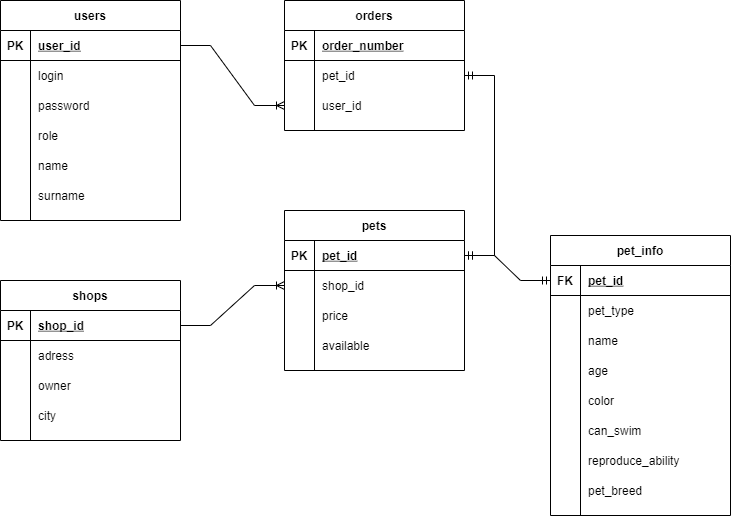
\includegraphics[scale=0.5]{img/Схема БД.drawio.png}
  \caption{Схема БД}
  \label{fig:image6}
\end{figure}

\newpage

\section{Архитектура программного обеспечения}

\hspace{0.6cm} В соответствии с техническим заданием будущее приложение должно иметь систему MVC(model, view, controller): веб-приложение(представление/view), базу данных(модель/model) и логику на серверную части(контроллер/controller). Основная цель применения этой концепции состоит в отделении бизнес-логики(модели) от её визуализации. За счёт такого разделения повышается возможность повторного использования кода.

\hspace{0.6cm} Основываясь на рисунке \ref{fig:image17} и модели MVC будет создаваться программа. Для каждого пункта доступного пользователю, а точнее: регистрация, авторизация, меню пользователя, меню продавца и меню администратора будет необходимо создать отдельный как контроллер, так и представление.

\hspace{0.6cm} Контроллер представляет из себя часть кода, которая отвечает за свое представление, передачу, получение и обработку данных с него, а так же взаимодействие с БД в случае необходимости добавления, удаления или изменения данных в ней.

\hspace{0.6cm} Функции работы с моделью (базой данных) храняться и реализовываются отдельно от контроллеров, однако предоставляют возможность к ним обращаться любым контроллерам. Каждая таблица при необходимости работы с ней имеет свое отдельное представление на уровне программы в виде класса или структуры данных. Это делается для более эфективной работы с данными.

\hspace{0.6cm} Представление связано со своим контроллером. Само представление является визуальной состовляеющей веб-приложения. Оно предоставялет возможность вводить пользователю данные, пользоваться функционалом посредством виджетов(кнопок), а также просматривать необходимую информацию.

\section{Выводы}

\hspace{0.6cm} В данном разделе были представлены схемы и диаграммы, представляющие структуру БД, а также описывающая логику её работы. Так же были показаны диаграммы работы системы ПО.

